\documentclass[11pt, oneside]{article}   	% use "amsart" instead of "article" for AMSLaTeX format

\usepackage{geometry}
 \geometry{
 a4paper,
 total={170mm,257mm},
 left=20mm,
 top=30mm,
 bottom=25mm, 
 }
 
%\usepackage{geometry}                		% See geometry.pdf to learn the layout options. There are lots.
%\geometry{letterpaper}                   		% ... or a4paper or a5paper or ... 
%\geometry{landscape}                		% Activate for rotated page geometry
%\usepackage[parfill]{parskip}    		% Activate to begin paragraphs with an empty line rather than an indent
\usepackage{graphicx}				% Use pdf, png, jpg, or eps§ with pdflatex; use eps in DVI mode
								% TeX will automatically convert eps --> pdf in pdflatex		

\usepackage{amssymb}
\usepackage{amsmath}
\usepackage{amsthm}
\usepackage{fancyhdr}
\usepackage[utf8]{inputenc}
\usepackage[english]{babel}
\usepackage{enumerate}
\usepackage{arcs}
\usepackage{array}
\usepackage{tabularx} 
\usepackage{tikz}
%SetFonts

%SetFonts

\usepackage[inline]{asymptote}


\pagestyle{fancy}
\fancyhf{}
\lhead{AMC8 solutions by WZ.}
%\rhead{}
%\rfoot{January 4, 2022}

\title{Solutions for Selected AMC8 Problems}
\author{wzuuzw}
\date{January 4, 2022}							% Activate to display a given date or no date

\begin{document}
\maketitle

\begin{enumerate}
\setlength\itemsep{3em}
\item  (AMC8 2015, p25) One-inch squares are cut from the corners of this 5 inch square. What is the area in square inches of the largest square that can fit into the remaining space?

\begin{center}
\begin{asy}
size(5cm);
draw((0,0)--(5, 0)--(5, 5)--(0, 5)--cycle);
filldraw((0,0)--(1, 0)--(1, 1)--(0, 1)--cycle, grey);
filldraw((0,4)--(1, 4)--(1, 5)--(0, 5)--cycle, grey);
filldraw((4,0)--(5, 0)--(5, 1)--(4, 1)--cycle, grey);
filldraw((4,4)--(5, 4)--(5, 5)--(4, 5)--cycle, grey);
draw((0, 3.618)--(3.618, 5)--(5, 1.372)--(1.372, 0)--cycle, blue);
dot((0, 4));
dot((0, 3.618));
dot((1,4));
dot((1, 5));
dot((3.618, 5));

label("$A$",(0, 3.618),W);
label("$B$",(0, 4),W);
label("$C$",(1, 4),S);
label("$D$",(1, 5),N);
label("$E$",(3.618, 5),N);
label("$F$",(0, 5),W);


\end{asy}
\end{center} 

\textbf{Solution:}
As illustrated above, the blue square is the largest square we want. It is attached to the corner square. The idea is to get the area of the blue square by subtracting the area of four corner triangles from the big square.

Suppose $AF = a, EF= b$, we have $a+b= 5$. To get the area of $\triangle AFE$, we have to calculate $ab$, which is done through similar triangles.

Since $\triangle ABC \sim \triangle CDE$, we have
\[\frac{AB}{CD} = \frac {BC}{DE} \quad \Rightarrow \quad \frac{a-1}{1}=\frac{1}{b-1}\quad \Rightarrow \quad (a-1)(b-1)= 1\quad \Rightarrow \quad ab = a+b.\]

Therefore, $ab = a+b = 5$. The area of the blue square is $25- 2ab = 25-10 = 15$.

\item (AMC8 2016, p22) Rectangle $DEFA$ is a $3\times 4$ rectangle with $DC=CB=BA$. What is the area of the ``bat wings" (shaded area)?

\begin{center}
\begin{asy}
size(5cm);
draw((0, 0)--(3, 0)--(3, -4)--(0, -4)--cycle);
filldraw((1, 0)--(1.5, -1)--(0, -4)--cycle, gray);
filldraw((2, 0)--(1.5, -1)--(3, -4)--cycle, gray);
label("$D$",(0, 0),N);
label("$C$",(1, 0),N);
label("$B$",(2, 0),N);
label("$A$",(3, 0),N);
label("$E$",(0, -4),S);
label("$F$",(3, -4),S);
label("$G$",(1.5, -1.2),S);
dot((1.5, -1));
draw((1.5, 0)--(1.5, -4), dashed+blue);
label("$x$",(1.5, -0.5),E);
label("$y$",(1.5, -2.5),E);
\end{asy}
\end{center}

\begin{itemize}
\item \textbf{Solution 1:}
The idea is to subtract the area of 4 triangles (white) from the area of the big rectangle. $S_{\triangle DCE} = S_{\triangle ABF}= 2$. We need to calculate the area of $\triangle BCG$ and $\triangle EFG$.

Suppose the heights of $\triangle BCG$ and $\triangle EFG$ are $x$ and $y$, respectively. Since $\triangle BCG \sim \triangle EFG$,  we have 
\[\frac{x}{y}=\frac{BC}{EF}=\frac{1}{3} \quad \Rightarrow \quad y=3x.\]

Together with $x+y=4$, we have $x=1, y=3$. 

Therefore, $S_{\triangle BCG}=\frac{x}{2}=\frac{1}{2}$,  $S_{\triangle EFG}=\frac{3y}{2}=\frac{9}{2}$, and the shaded area is
\[12-2-2-\frac{1}{2}-\frac{9}{2}=3.\]

\item \textbf{Solution 2:}
We solve this problem using area equations. Since $\triangle BCG \sim \triangle EFG$, 
\[\frac{BC}{FE}=\frac{CG}{GF}=\frac{1}{3},\qquad \Rightarrow \qquad \frac{S_{\triangle BCG}}{S_{\triangle EFG}}=\frac{1}{9},\quad \frac{S_{\triangle BCG}}{S_{\triangle BGF}}=\frac{1}{3}. \] 

Assume $S_{\triangle BCG}=a$ , then $S_{\triangle EFG}=9a, S_{\triangle CGE}= S_{\triangle BGF}=3a.$

Since $AB=BC=CD$, we have $S_{\triangle ABF}=S_{\triangle CDE}=S_{\triangle BCF}=4a$. Totally, \[S_{ADEF}=1a+9a+3a+3a+4a+4a=12, \qquad\Rightarrow\qquad a=\frac{1}{2}.\]

Finally, the area of the shaded region is $3a+3a=3$. 



\end{itemize}

\item (AMC8 2020, p21) A game board consists of 64 squares that alternate in color between black and white. The figure below shows square $P$ in the bottom row and square $Q$ in the top row. A marker is placed at $P$. A step consists of moving the marker onto one of the adjoining white squares in the row above. How many 7-step paths are there from $P$ to $Q$? (The figure shows a sample path.)
\begin{center}


\begin{asy}
size(5cm);
for(int i=0; i<9; ++i){
    draw((0, -i)--(8, -i));
    draw((i, 0)--(i, -8));
}

for(int j=0; j<8; ++j)
for(int i=0; i<8; ++i) {
    if ((i+j)%2 == 1) {
        filldraw((i, -j)--(i+1, -j)--(i+1, -j-1)--(i, -j-1)--cycle, gray);
    }
}

real [][] c= {{6.5, -0.5}, {5.5, -1.5}, {6.5, -2.5}, {5.5, -3.5}, {4.5, -4.5}, {5.5, -5.5}, {6.5, -6.5}};
for(int i=0; i<7; ++i){
    real x=c[i][0];
    real y=c[i][1];
    draw(circle((x, y), 0.4));
}
label("$P$", (5.5, -7.5));
label("$Q$", (6.5, -0.5));
label("$A$", (4.5, -6.5));
label("$B$", (6.5, -6.5));
label("$C$", (5.5, -1.5));
label("$D$", (7.5, -1.5));
\end{asy}
\end{center}

\textbf{Solution:}
We solve this problem by dynamic programming. A key observation is that if he number of paths from $Q$ to $A$  is $f(A)$, and the number of path from  $Q$ to $B$ is $f(B)$, then the total number of paths from $Q$ to $P$ is $f(A)+f(B)$. Apparently, $f(Q)=1$.

For the 2 adjacent white squares $C$ and $D$ below $Q$, we have $f(C) = f(Q) = 1, f(D) = f(Q) = 1$.

In order to reach $P$ in 7 steps from $Q$, we must move downward for every step. Therefore, starting from $Q$, there is no path to the 3 white squares in the left of the top row. Now, from top to bottom, we are able to mark the number of paths from $Q$ to every white square, as illustrated below. The number of paths from $Q$ to $P$ is $14 + 14 = 28$.

\begin{center}
\begin{asy}
size(5cm);
for(int i=0; i<9; ++i){
    draw((0, -i)--(8, -i));
    draw((i, 0)--(i, -8));
}

for(int j=0; j<8; ++j)
for(int i=0; i<8; ++i) {
    if ((i+j)%2 == 1) {
        filldraw((i, -j)--(i+1, -j)--(i+1, -j-1)--(i, -j-1)--cycle, gray);
    }
}

real [][] c= {{6.5, -0.5}, {5.5, -1.5}, {6.5, -2.5}, {5.5, -3.5}, {4.5, -4.5}, {5.5, -5.5}, {6.5, -6.5}};
for(int i=0; i<7; ++i){
    real x=c[i][0];
    real y=c[i][1];
    draw(circle((x, y), 0.4));
}
label("$28$", (5.5, -7.5));

label("$1$", (6.5, -0.5));
label("$0$", (0.5, -0.5));
label("$0$", (2.5, -0.5));
label("$0$", (4.5, -0.5));

label("$0$", (1.5, -1.5));
label("$0$", (3.5, -1.5));
label("$1$", (5.5, -1.5));
label("$1$", (7.5, -1.5));

label("$0$", (0.5, -2.5));
label("$0$", (2.5, -2.5));
label("$1$", (4.5, -2.5));
label("$2$", (6.5, -2.5));

label("$0$", (1.5, -3.5));
label("$1$", (3.5, -3.5));
label("$3$", (5.5, -3.5));
label("$2$", (7.5, -3.5));

label("$0$", (0.5, -4.5));
label("$1$", (2.5, -4.5));
label("$4$", (4.5, -4.5));
label("$5$", (6.5, -4.5));

label("$1$", (1.5, -5.5));
label("$5$", (3.5, -5.5));
label("$9$", (5.5, -5.5));
label("$5$", (7.5, -5.5));

label("$1$", (0.5, -6.5));
label("$6$", (2.5, -6.5));
label("$14$", (4.5, -6.5));
label("$14$", (6.5, -6.5));
\end{asy}
\end{center}

\item (AMC8 2020, p20) A scientist walking through a forest recorded as integers the height of 5 trees standing in a row. She observed that that each tree was twice as tall or half as tall as the one to its right. Unfortunately some of her data was lost when rain fell on her notebook. Her notes are shown below, with blanks indicating the missing numbers. Based on her observation, the scientist was able to reconstruct the lost data. What was the average height of the trees, in meters?
\begin{center}

\renewcommand{\arraystretch}{1.5}
\begin{tabular}{|c|c|}
\hline
Tree 1 &  \underline{\quad} meters\\
Tree 2 &11 meters\\
Tree 3 &  \underline{\quad} meters\\
Tree 4 &  \underline{\quad} meters\\
Tree 5 &  \underline{\quad} meters\\
\hline
Average height &  $\underline{\quad}.2$ meters\\
\hline
\end {tabular}
\end{center}

\textbf{Solution:}
We solve this problem using tree diagram. Because the heights are integers, both Tree 1 and Tree 3 should be 22 meters. We show the tree diagram as follows.

\begin{center}
\begin{asy}
size(11cm);
draw(box((0.4, 0), (2.6, 1)));
draw(box((0, -1), (-2, -2)));
draw(box((3, -1), (5, -2)));
draw(box((3, -3), (1, -4)));
draw(box((5, -3), (7, -4)));
draw(box((0, -3), (-2, -4)));

draw((-4,-0.5)--(7,-0.5), dashed+blue);
draw((-4,-2.5)--(7,-2.5), dashed+blue);
draw((-4,-4.5)--(7,-4.5), dashed+blue);

label("Tree 1, 2, 3", (-4,0.5));
label("Tree 4", (-4,-1.5));
label("Tree 5", (-4,-3.5));
label("Total", (-4,-5));

label("22, 11, 22", (1.5, 0.5));
label("11", (-1, -1.5));
label("44", (4, -1.5));

label("22", (-1, -3.5));
label("22", (2, -3.5));
label(" 88", (6, -3.5));
label("88", (-1, -5));
label("121", (2, -5));
label(" 187", (6, -5));

draw((1.5, 0)--(-1, -1));
draw((1.5, 0)--(4, -1));
draw((4, -2)--(2, -3));
draw((4, -2)--(6, -3));
draw((-1, -2)--(-1, -3));
\end{asy}
\end{center}

Among the 3 possible values 88, 121, and 187, only 121 results an average of 24.2, which is the correct answer!

\item (AMC8 2015, p19) A triangle with vertices as $A=(1, 3), B=(5, 1),$ and $C=(4,4)$ is plotted on a $6\times 5$ grid. What fraction of the grid is covered by the triangle?

\begin{center}
\begin{asy}
size(5cm);
import math;
add(grid(6,5));
draw((0,0)--(7,0), arrow=Arrow());
draw((0,0)--(0,6), arrow=Arrow());
draw((1,3)--(4,4)--(5,1)--cycle);
label("$A$", (1,3), SW);
label("$B$", (5,1), SE);
label("$C$", (4,4), NE);
label("$x$", (7,0), S);
label("$y$", (0,6), W);
\end{asy}
\end{center}

\item (AMC8 2022, p25) A cricket randomly hops between $4$ leaves, on each turn hopping to one of the other $3$ leaves with equal probability. After $4$ hops what is the probability that the cricket has returned to the leaf where it started?
\begin{center}
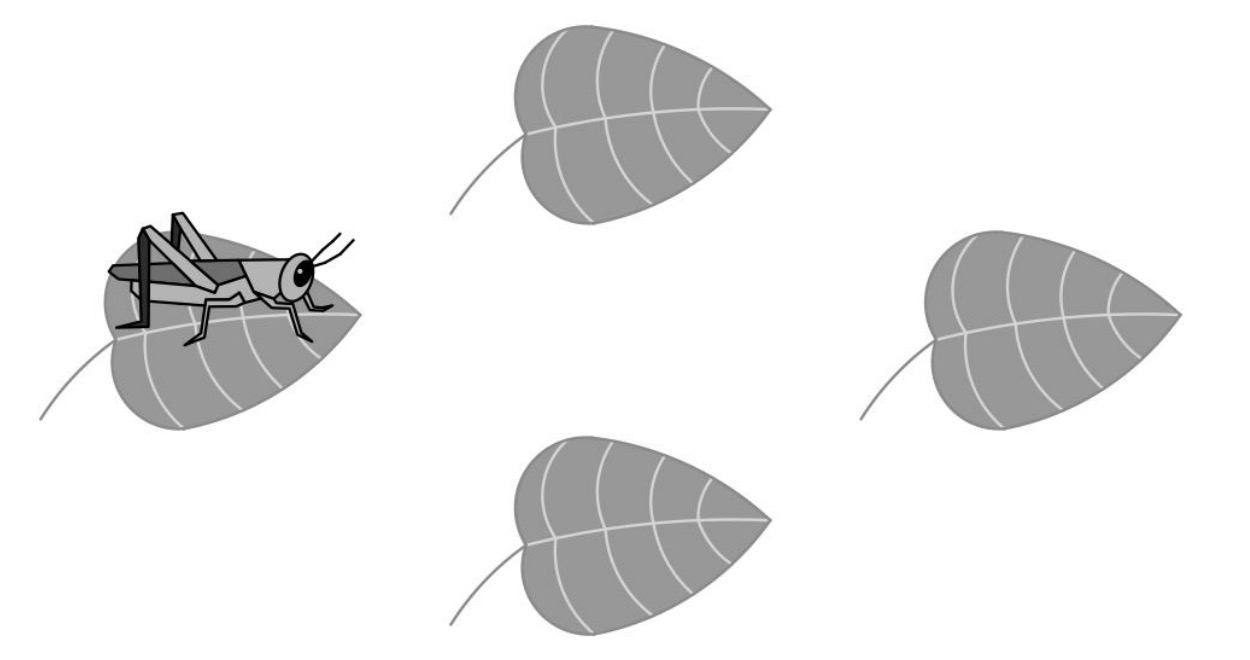
\includegraphics[scale=0.3]{imgs/2022_AMC_8_Problem_25.jpeg}
\end{center}

\textbf{Solution:}

We solve this problem using tree diagram and dynamic programming. We analyze this problem by stages.

Stage 1): If the cricket jumps 1 hop, there are 3 different ways. \\
Stage 2): If the cricket jumps 2 hops, there are $3^2=9$ different ways. Among the 9 ways, there are 3 ways leading to the start leaf.  The rest 6 ways don't lead to the start leaf. We illustrate the 2-hop scenario in the tree diagram, where black nodes represent the start leaf, and white nodes represent other leaves.\\
\begin{center}
\begin{asy}
size(6cm);
for (int i=0; i<9; ++i) {
    int x = (int) (i/3);
    draw((i,0)--(x*3+1,2));
    if (i%3 == 0) { 
        filldraw(circle((i, 0), 0.2), black, black); 
    } else {
        filldraw(circle((i, 0), 0.2), white, black);
    }
}

for (int i=0; i<3; ++i) {
    draw((i*3+1,2)--(4,4));
    filldraw(circle((i*3+1, 2), 0.2), white, black);
}

filldraw(circle((4,4),0.2), black, black);

draw((-1,-0.5)--(10,-0.5), dashed);
draw((-1,1.5)--(10,1.5), dashed);
label("\small 1 hop", (8.6,2.2), E);
label("\small 2 hops", (8.6,0.2), E);
\end{asy}
\end{center}

Stage 3): If the cricket jump 3 hops, there are $3^3=27$ different ways.  A key observation is: Only a path that doesn't lead to the start leaf in stage 2 can have a path leading to the start leaf in stage 3. Among the 27 ways, there are 6 ways leading to the start leaf. The rest 21 ways don't lead to the start leaf, obviously.\\
Stage 4): If the cricket jumps 4 hops, there are $3^4=81$ different ways. From stage 3, we know that there are 21 ways leading to the start leaf.


Therefore, the probability is $\frac{21}{81}=\frac{7}{27}$.

\item  Test
\begin{center}
\begin{asy}
import patterns;
size(5cm);

add("shd1", hatch(H=2mm, dir=SE, red));

fill(arc((0,0), r=2, angle1=-40, angle2=40)--arc((3,0),r=2, angle1=140, angle2=220)--cycle, pattern("shd1"));

draw(circle((0,0),2));
draw(circle((3,0),2));
draw(circle((1.5,-2.56),2));

\end{asy}
\end{center}

\end{enumerate}
\end{document}  






